\documentclass{standalone}
\usepackage{tikz}
\usetikzlibrary{arrows.meta, positioning}

\begin{document}
\begin{tikzpicture}[node distance=2cm, auto]
    % Definir nodos para los módulos principales
    \node (ui) [draw, rectangle, fill=blue!20] {Interfaz de Usuario\\(ControlAGPropio)};
    \node (vis) [draw, rectangle, fill=green!20, right=of ui] {Sistema de Visualización\\(LineRenderer, Prefabs)};
    \node (geneticsharp) [draw, rectangle, fill=red!20, below=of ui] {Módulo AG GeneticSharp\\(GAController, TspFitness)};
    \node (propio) [draw, rectangle, fill=yellow!20, below=of vis] {Módulo AG Propio\\(AlgoritmoGenetico, Cromosoma)};
    \node (ciudades) [draw, rectangle, fill=orange!20, left=of geneticsharp] {Generación de Ciudades\\(Ciudad, TspCity)};
    \node (rutas) [draw, rectangle, fill=purple!20, right=of propio] {Representación de Rutas\\(DrawRoute, LineRenderer)};

    % Dibujar conexiones entre módulos
    \draw[->] (ui) -- (geneticsharp) node[midway, above] {Configura};
    \draw[->] (ui) -- (propio) node[midway, above] {Configura};
    \draw[->] (geneticsharp) -- (ciudades) node[midway, left] {Genera};
    \draw[->] (propio) -- (ciudades) node[midway, left] {Genera};
    \draw[->] (ciudades) -- (vis) node[midway, above] {Proporciona datos};
    \draw[->] (geneticsharp) -- (rutas) node[midway, right] {Actualiza};
    \draw[->] (propio) -- (rutas) node[midway, right] {Actualiza};
    \draw[->] (rutas) -- (vis) node[midway, below] {Renderiza};
\end{tikzpicture}
\end{document}